\section{Flujo sobre el dispositivo objetivo}

Con el comportamiento verificado se sintetizó el diseño para el dispositivo \texttt{xc7a35tcpg236-1}. En esta etapa \tech{Vivado} transforma los operadores y registros de la descripción RTL en una red de recursos disponibles en la \tech{Artix-7}. La síntesis terminó correctamente, como se muestra en la figura~\ref{fig:synthesis}, y permitió avanzar a la implementación.

\begin{figure}[H]
	\centering
	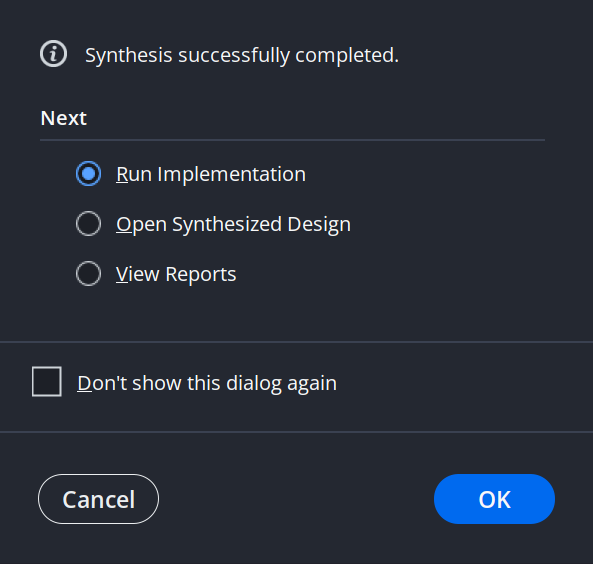
\includegraphics[width=0.43\textwidth]{img/synthesis_successful.png}
	\caption{Finalización correcta de la síntesis.}
	\label{fig:synthesis}
\end{figure}

Durante la implementación se determina la ubicación de los recursos y el ruteo de sus conexiones. El proceso incorpora las restricciones de pines y reloj y genera el diseño sobre el que se efectúa el análisis temporal posterior al ruteo. La figura~\ref{fig:implementation} documenta su finalización.

\begin{figure}[H]
	\centering
	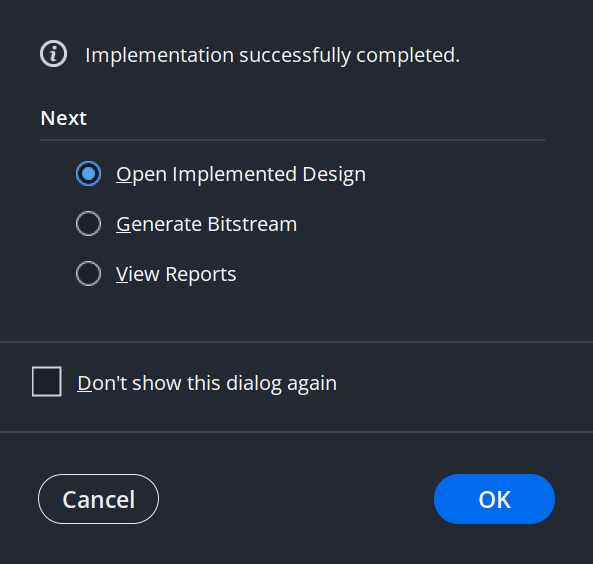
\includegraphics[width=0.43\textwidth]{img/implementation_successful.png}
	\caption{Finalización correcta de la ubicación y el ruteo.}
	\label{fig:implementation}
\end{figure}

\section{Del esquema RTL a los recursos físicos}

El esquema implementado del top conserva el recorrido de la vista RTL: entradas, sincronizadores, registros, ALU y salidas. La diferencia es el nivel de detalle. Los bancos aparecen descompuestos en registros individuales y se incorporan buffers de entrada, salida y distribución del reloj.

\begin{figure}[H]
	\centering
	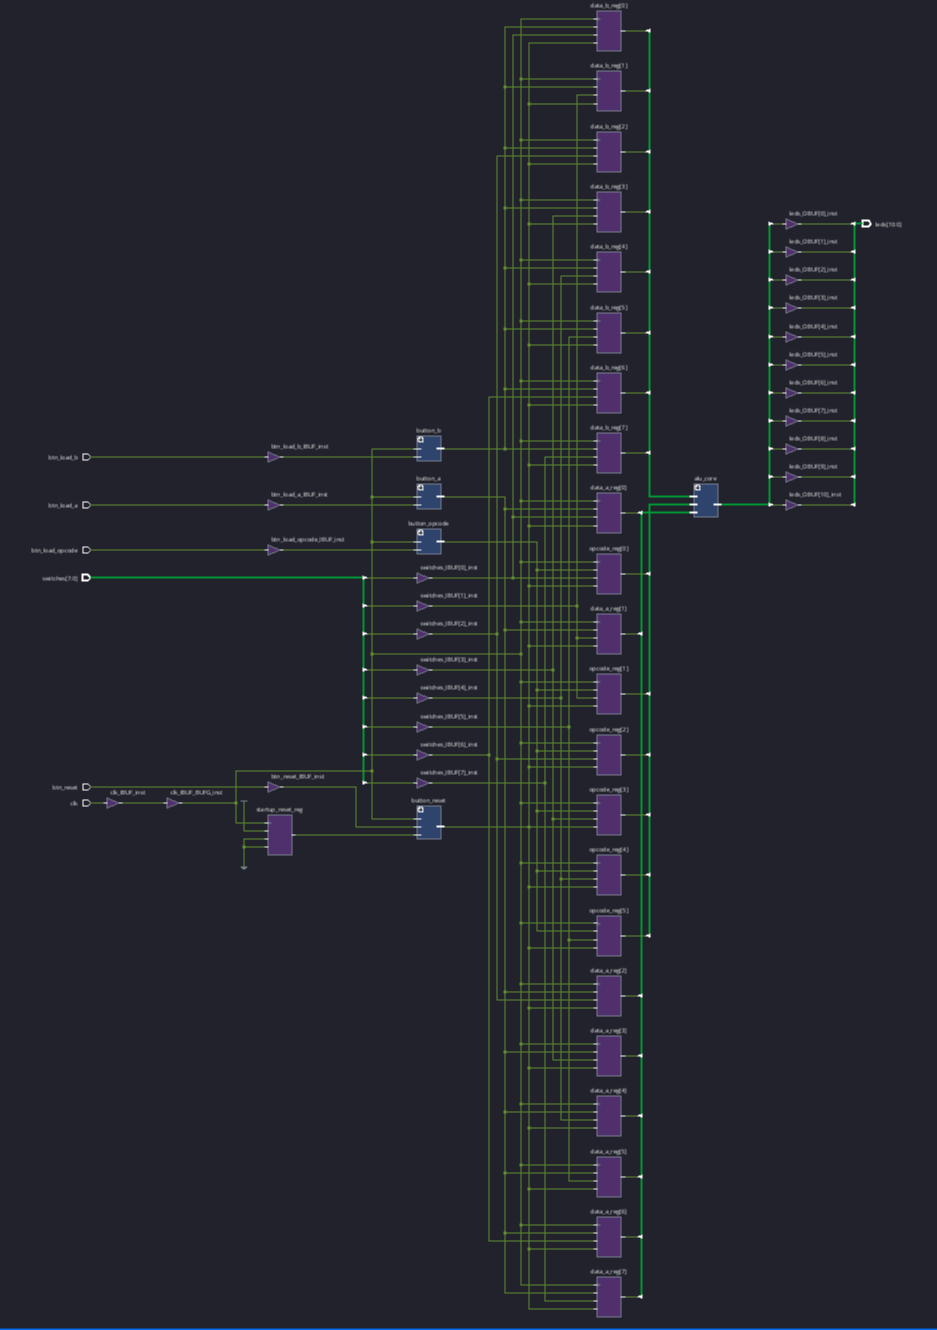
\includegraphics[height=0.72\textheight]{img/schematic_top_implementation.png}
	\caption{Recursos y conexiones del módulo superior implementado.}
	\label{fig:top-impl}
\end{figure}

Al abrir la ALU se observa cómo se resolvieron las operaciones en la tecnología del dispositivo. Las expresiones del código no se convierten necesariamente en compuertas individuales: la herramienta combina funciones dentro de las \tech{LUT} y emplea cadenas dedicadas \tech{CARRY4} para la aritmética. La figura~\ref{fig:alu-impl} explica, por tanto, la diferencia entre los operadores abstractos de la vista RTL y la red implementada.

\begin{figure}[H]
	\centering
	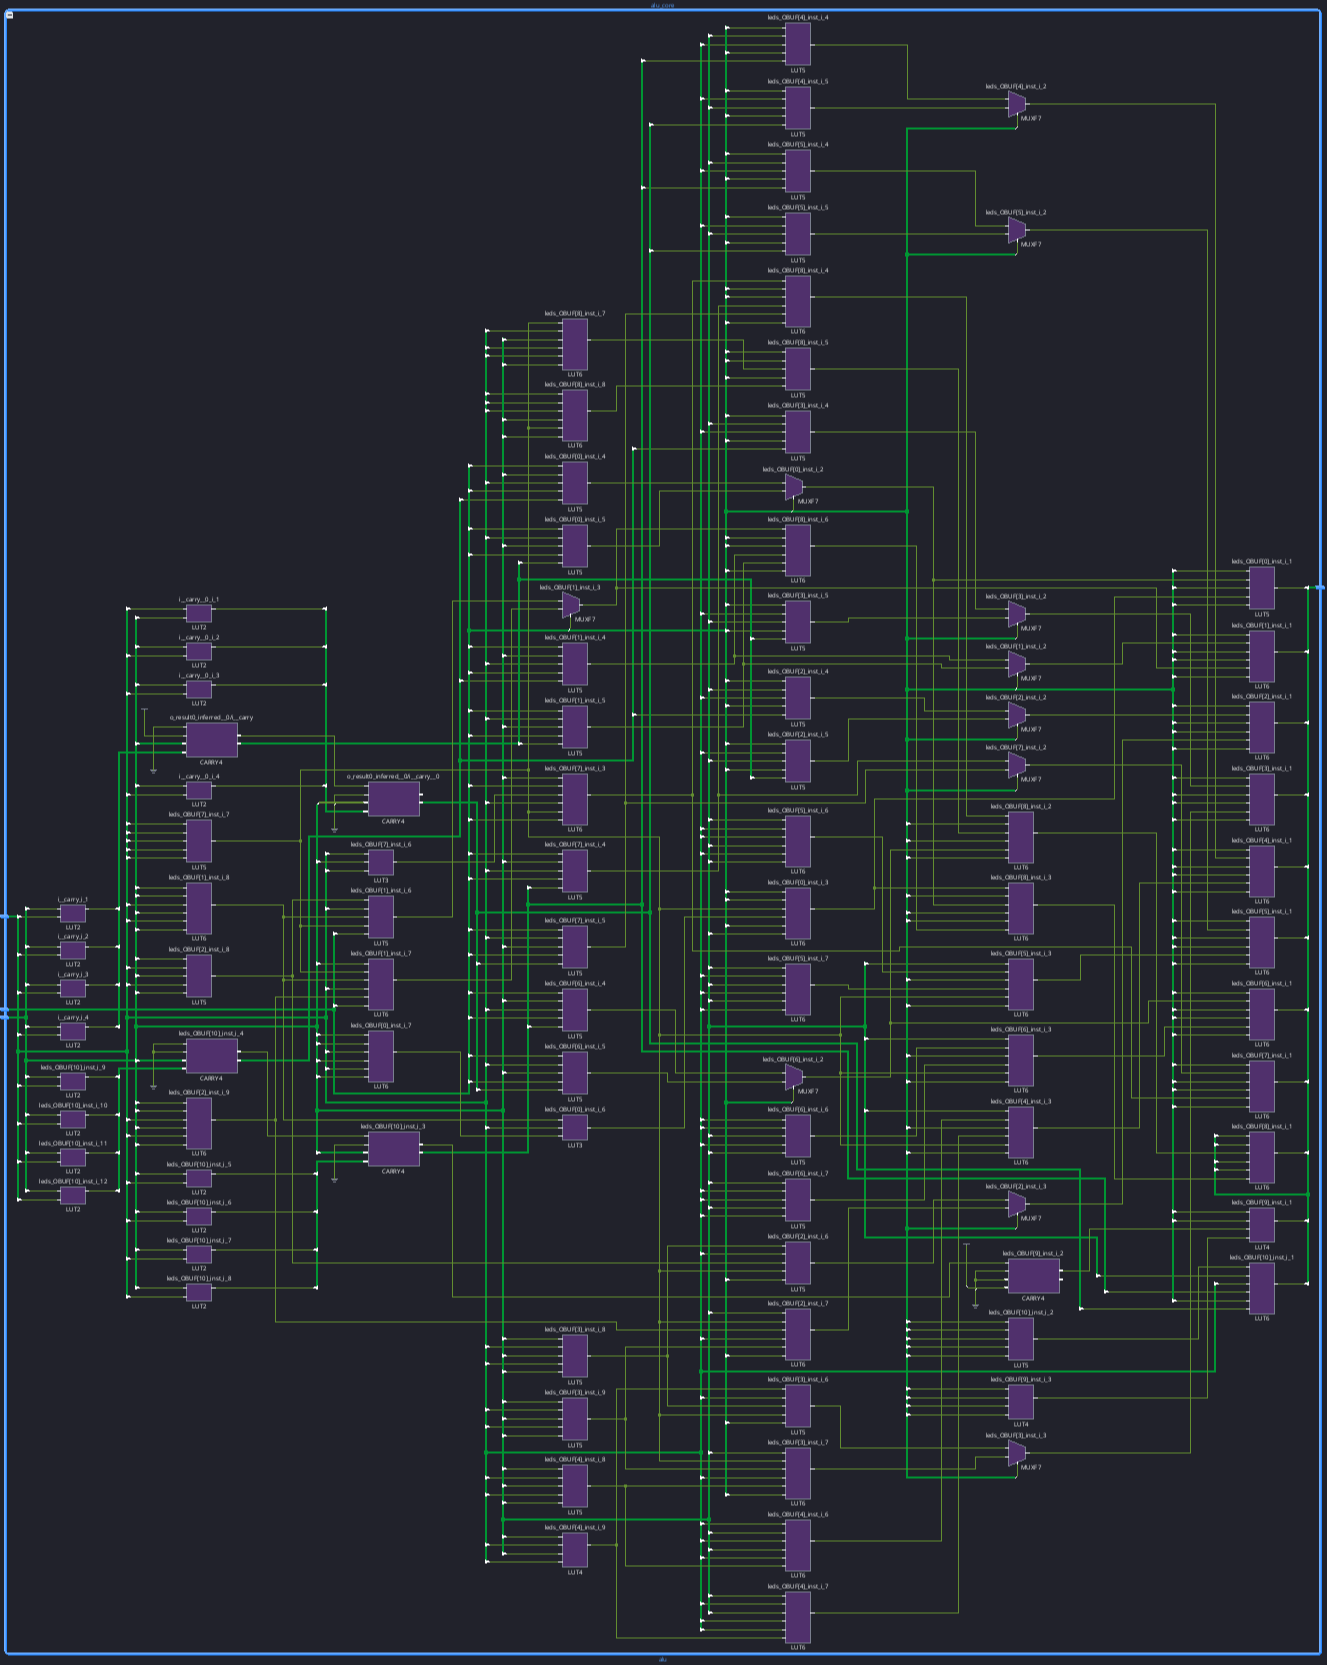
\includegraphics[height=0.72\textheight]{img/schematic_alu_implementation.png}
	\caption{Implementación de la ALU mediante LUT, multiplexores y cadenas de acarreo.}
	\label{fig:alu-impl}
\end{figure}

En el sincronizador la correspondencia es más directa. Los dos registros de la descripción se implementan con dos flip-flops \tech{FDRE}, con un reloj compartido y conexión en serie.

\begin{figure}[H]
	\centering
	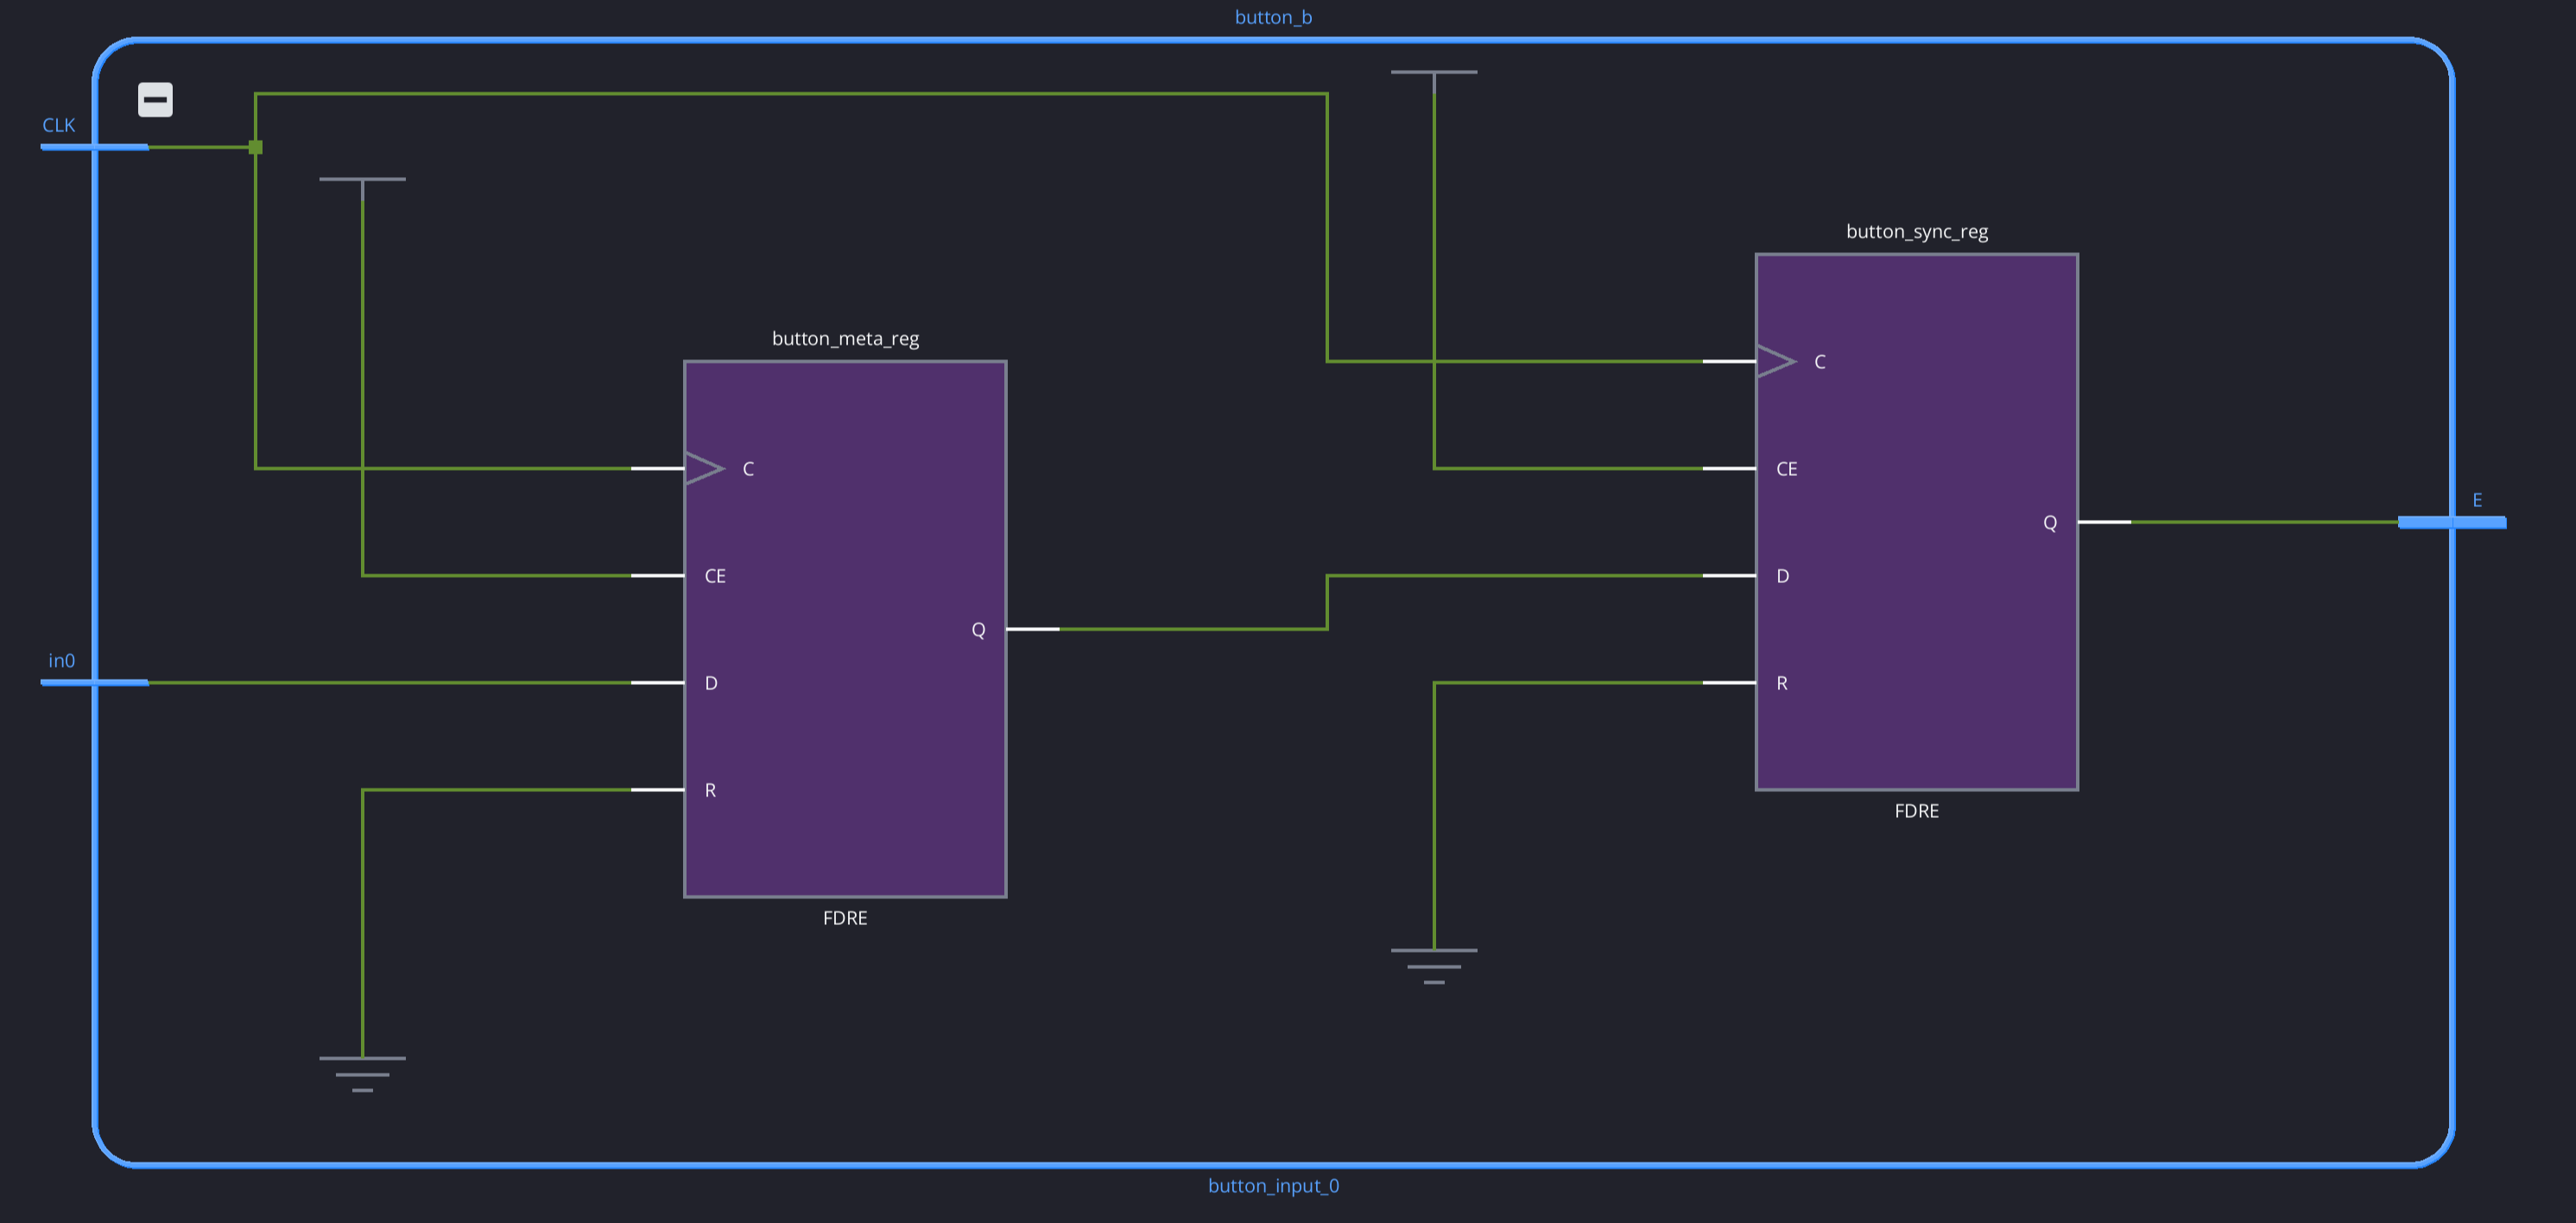
\includegraphics[width=\textwidth]{img/schematic_button_implementation.png}
	\caption{Dos flip-flops FDRE implementan las etapas del sincronizador.}
	\label{fig:button-impl}
\end{figure}

\section{Utilización de recursos}

El reporte de utilización cuantifica el costo del circuito. Los resultados se resumen en la tabla~\ref{tab:resources}.

\begin{table}[H]
\centering
\begin{tabular}{lrrr}
\toprule
\textbf{Recurso} & \textbf{Utilizado} & \textbf{Disponible} & \textbf{Utilización} \\
\midrule
LUT & 76 & 20.800 & \SI{0,37}{\percent} \\
Flip-flops & 31 & 41.600 & \SI{0,07}{\percent} \\
I/O & 24 & 106 & \SI{22,64}{\percent} \\
\bottomrule
\end{tabular}
\caption{Recursos utilizados en la Artix-7.}
\label{tab:resources}
\end{table}

\begin{figure}[H]
	\centering
	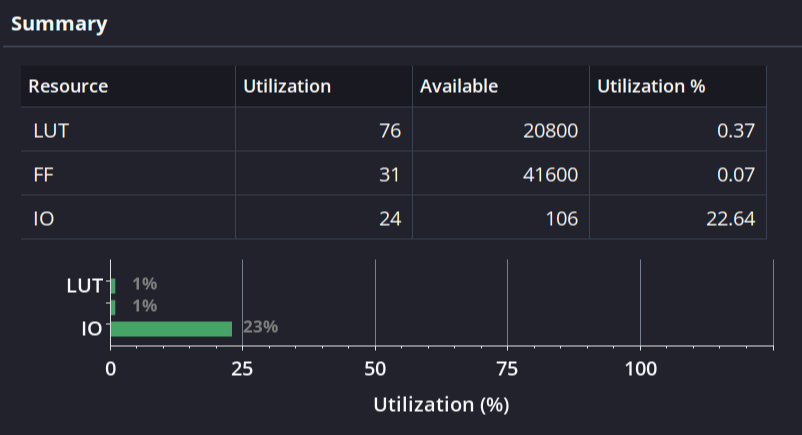
\includegraphics[width=0.80\textwidth]{img/utilization_summary.png}
	\caption{Resumen de utilización de recursos.}
	\label{fig:util-summary}
\end{figure}

Los 31 flip-flops coinciden con la estructura prevista: los registros de A, B y opcode requieren 22 bits; los cuatro sincronizadores agregan ocho, y el reset de arranque utiliza uno. Los 24 I/O se corresponden con ocho switches, cuatro botones, un reloj y once LED. Este contraste permite validar el reporte contra las decisiones de diseño.

La vista jerárquica indica que 75 de las 76 LUT pertenecen al núcleo y que este no contiene registros, como corresponde a su carácter combinacional. La fila del top ya incluye los recursos de sus submódulos y no debe sumarse otra vez. También aparecen once multiplexores F7 y un buffer global de reloj.

\begin{figure}[H]
	\centering
	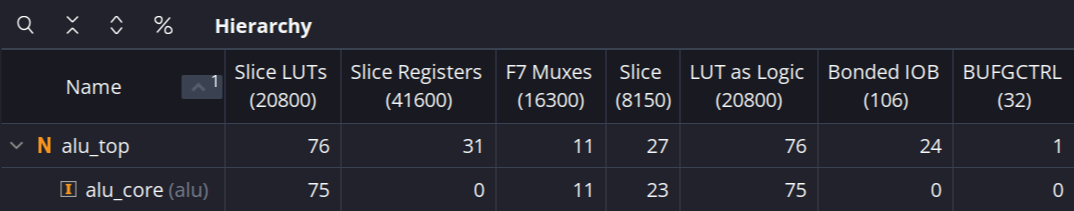
\includegraphics[width=\textwidth]{img/utilization_hierarchy.png}
	\caption{Distribución de recursos entre el módulo superior y la ALU.}
	\label{fig:util-hierarchy}
\end{figure}

Finalmente, la vista \textit{Device} de la figura~\ref{fig:device} permite ubicar el circuito dentro de la estructura física de la FPGA. Los porcentajes se toman del reporte de utilización, ya que el tamaño aparente de los elementos en esta vista depende de la representación gráfica.

\begin{figure}[H]
	\centering
	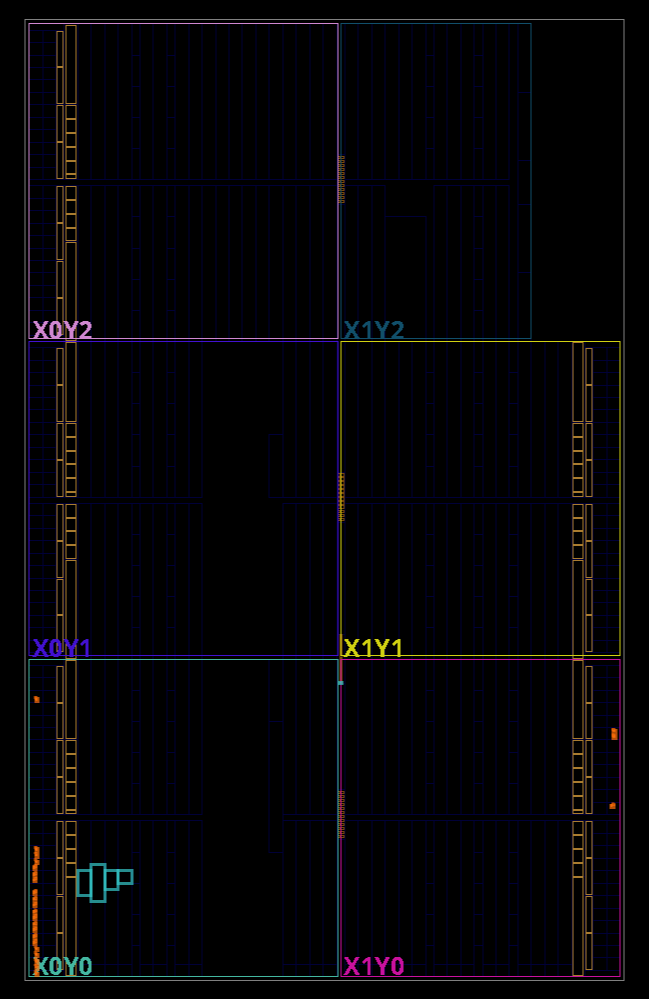
\includegraphics[height=0.73\textheight]{img/device.png}
	\caption{Distribución física del circuito en la vista Device.}
	\label{fig:device}
\end{figure}
